\documentclass[../../../interview-questions.tex]{subfiles}

\begin{document}

\subsection{Spring Bean的生命周期}


Bean 的生命周期主要为实例化、属性填充、初始化和销毁 4 个阶段,加上类加载和使用阶段,整个流程如下:

\begin{figure}[htbp]
	\centering
	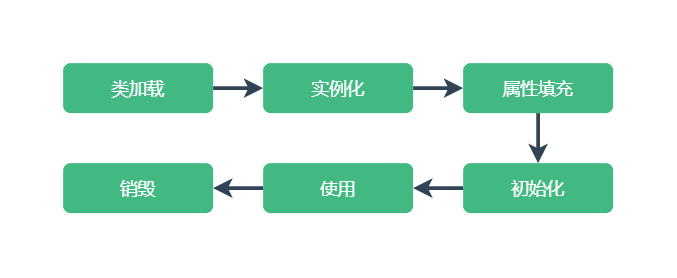
\includegraphics[scale=0.5]{spring-bean-lifecycle.png}
	\caption{Spring Bean生命周期}
	\label{fig:spring-bean-lifecycle}
\end{figure}

https://www.modb.pro/db/436912

Spring Bean的生命周期分为四个阶段和多个扩展点。扩展点又可以分为影响多个Bean和影响单个Bean。整理如下:
四个阶段

\begin{enumerate}
    \item {实例化 Instantiation}
    \item {属性赋值 Populate}
    \item {初始化 Initialization}
    \item {销毁 Destruction}
\end{enumerate}

\paragraph{Spring Bean生命周期的扩展点}

扩展点分为容器级与对象级,如果是容器级的话你实现的那个扩展点操作会应用到容器内所有的Bean,如果是Bean级别的话就只能影响那个Bean。所谓Bean生命周期的扩展点,就是Spring留给我们干预Bean生命周期的回调。这个比较好理解,因为我们把对象及其依赖的管理托管给了Spring,但是我们又要在这个过程中进行干预,所以spring就必须在管理Bean的各个阶段留有接入点。Spring Bean扩展点分为2类,一类影响单个Bean的扩展点,一类影响多个Bean的扩展点。影响多个Bean的扩展点:

\begin{enumerate}
    \item{BeanPostProcessor}
    \item {InstantiationAwareBeanPostProcessor}
\end{enumerate}

对象级扩展点作用于单个bean,只对单个bean起作用。影响单个Bean扩展点:

\begin{enumerate}
    \item {BeanNameAware}
    \item {BeanClassLoaderAware}
    \item {BeanFactoryAware}
    \item {EnvironmentAware}
    \item {EmbeddedValueResolverAware}
    \item {ApplicationContextAware(ResourceLoaderAware ApplicationEventPublisherAware MessageSourceAware)}
\end{enumerate}

https://shusheng007.top/2022/10/12/1-17/

\end{document}





